\documentclass[10pt]{beamer}

% \usepackage[table,xcdraw]{xcolor}
\usepackage[square,numbers]{natbib}
\usepackage{graphicx}
\usepackage{svg}
\usepackage{pgfplots}
\usepgfplotslibrary{dateplot}

% \usetheme[progressbar=frametitle]{metropolis}
\usecolortheme{Imperial}
\usepackage{appendixnumberbeamer}

\usepackage{booktabs}
\usepackage[scale=2]{ccicons}


\usepackage{pgfplots}
\usepgfplotslibrary{dateplot}
\usepackage{xspace}
\newcommand{\themename}{\textbf{\textsc{metropolis}}\xspace}

\usepackage{amsfonts, amsmath, amsthm, amssymb}
\usepackage{bbm}
\usepackage{bm}
\usepackage{mathtools}
\usepackage[ruled,vlined]{algorithm2e}
\newlength{\commentWidth}
\setlength{\commentWidth}{7cm}
\newcommand{\atcp}[1]{\tcp*[r]{\makebox[\commentWidth]{#1\hfill}}}
\usepackage{setspace}
\usepackage[utf8]{inputenc}

\newcommand*{\QEDA}{\hfill\ensuremath{\blacksquare}}%
\newcommand*{\QEDB}{\hfill\ensuremath{\square}}%

\usepackage{tikz}
\usepackage{tikz-qtree}
\usepackage{forest}
\usetikzlibrary{trees} % this is to allow the fork right path

\setbeamertemplate{itemize items}[circle]
\setbeamertemplate{enumerate items}[default]
\usefonttheme[onlymath]{serif}


\title{\textbf{Transporte Ótimo para Redes Neurais}}
\subtitle{}
% \date{\today}
\date{}
\author{\textbf{Autor:} Davi Sales Barreira \\\hfill\\}
\institute{
\includegraphics[height=0.55cm]{emaplogo.png}}
\titlegraphic{
\includegraphics[height=0.35cm]{emaplogo-neg.png}}


\usepackage{caption}
\captionsetup[figure]{font=footnotesize}

\begin{document}

\maketitle

\begin{frame}{Sumário}
	\setbeamertemplate{section in toc}[sections numbered]
	\setbeamertemplate{subsection in toc}[subsections numbered]
	% \setbeamerfont{section in toc}{size=\normal}
	\setbeamerfont{subsection in toc}{size=\small}
	% \tableofcontents[hideallsubsections]
	\tableofcontents[sectionstyle=show, subsectionstyle=show]
\end{frame}

\AtBeginSection{}
\section[Introdução]{Introdução}
\begin{frame}[fragile]{Ideia Geral}

	Transporte Ótimo (OT) é uma área da matemática que estuda o problema
	de transportar ``massa'' em uma configuração para outra
	enquanto se miniza o custo de transporte.

	\vspace{3mm}
	Apesar de parecer um problema bastante específico, a ideia de se transportar objetos de maneira ótima
	é bastante ubíqua e possui diversas utilidades.

	\vspace{3mm}
	OT tem aparecido em diversas aplicações recentes de Machine Learning, como:
	\textbf{\textit{transfer learning, clustering}, redução de dimensionalidade,
		modelos generativos}, entre outros.

\end{frame}

\begin{frame}[fragile]{Ideia Geral}

	\begin{figure}[H]
		\centering
		\def\svgscale{0.7}
		\includesvg[inkscapelatex=false]{Figures/citations_distribution2}
		\caption{
			Gráficos com a evolução do número de publiações
			relacionadas a Transporte Ótimo com Machine Learning
			\citep{sales2021optimal}.}
		\label{fig:pub}
	\end{figure}

\end{frame}

\begin{frame}[fragile]{Ideia Geral}

	A solução de um problema de Transporte Ótimo sempre resulta
	em dois subprodutos, o \textbf{plano (mapa)} ótimo de transporte
	e o \textbf{custo mínimo} para realizar o transporte.

	\vspace{3mm}
	A maioria das aplicações em ML utiliza o custo mínimo para
	definir uma métrica de distância (e.g. Wasserstein). Porém,
	existem aplicações como Transfer Learning que utlilizam
	os mapas ótimos \citep{sales2021optimal}.

	\vspace{3mm}
	Nesta apresentação vamos focar na aplicação mais celebrada
	de OT em redes neurais, as chamadas
	\textbf{Wasserstein Generative Neural Networks} \citep{arjovsky2017wasserstein}.

\end{frame}

\AtBeginSection{}
\section[Teoria de Transporte Ótimo]{Teoria de Transporte Ótimo}
\subsection[Teoria OT]{Monge \& Kantorovich}
\begin{frame}[fragile]{Teoria OT - Monge \& Kantorovich}

	\textbf{Problema de Monge} -
	Qual a maneira ótima de transporta massa de uma configuração
	para outra?
	\vspace{3mm}

	\begin{figure}[H]
		\centering
		\def\svgscale{0.4}
		\includesvg[inkscapelatex=false]{Figures/mongeproblem.svg}
		\caption{Massa não pode ser separada.}
		\label{fig:mongeproblem}
	\end{figure}

	\textbf{Kantorovich Problem} -
	Relaxação do problema original de Monge.
	\vspace{3mm}

	\begin{figure}[H]
		\centering
		\def\svgscale{0.4}
		\includesvg[inkscapelatex=false]{Figures/kantorovichproblem.svg}
		\caption{Massa pode ser separada.}
		\label{fig:kantorovichproblem}
	\end{figure}

\end{frame}


\begin{frame}[fragile]{Teoria OT - Monge \& Kantorovich}

	\begin{definition}[Problema de Monge]
		Dadas duas medidas de probabilidade $\mu \in \mathcal P(X)$,
		$\nu \in \mathcal{P}(Y)$ e uma função de custo
		$c:X\times Y \to[0,+\infty]$, resolva:
		\begin{flalign}
			(MP)     &  &
			\inf
			\left\{
			\int_{X} c(x,T(x))d\mu \quad : \quad
			T_\# \mu = \nu
			\right\} &  &
		\end{flalign}

	\end{definition}

	\begin{figure}[H]
		\centering
		\def\svgscale{0.45}
		\includesvg[inkscapelatex=false]{Figures/monge_map_example.svg}
		\caption{Exemplo de dois problemas de Transporte Ótimo.}
		\label{fig:monge_map_example}
	\end{figure}

\end{frame}

\begin{frame}[fragile]{Teoria OT - Monge \& Kantorovich}

	\begin{definition}[Acoplamento (\textit{Coupling})]
		Sejam $(X,\mu)$ e $(Y,\nu)$ espaços de probabilidade. Para
		$\gamma \in \mathcal{P}(X\times Y)$, dizemos que $\gamma$
		é um acoplamento de $(\mu,\nu)$ se $(\pi_X)_\# \gamma = \mu$
		e $(\pi_Y)_\# \gamma = \nu$. Chamamos $\Pi(\mu,\nu)$
		do conjunto de \textbf{Planos de Transporte}:
		\begin{equation}
			\Pi(\mu,\nu) :=
			\left \{
			\gamma \in \mathcal{P}(X \times Y) \ :
			\ (\pi_X)_\# \gamma = \mu \quad
			\text{and} \quad
			(\pi_Y)_\# \gamma = \nu
			\right \}
		\end{equation}
	\end{definition}

	\begin{figure}[H]
		\begin{center}
			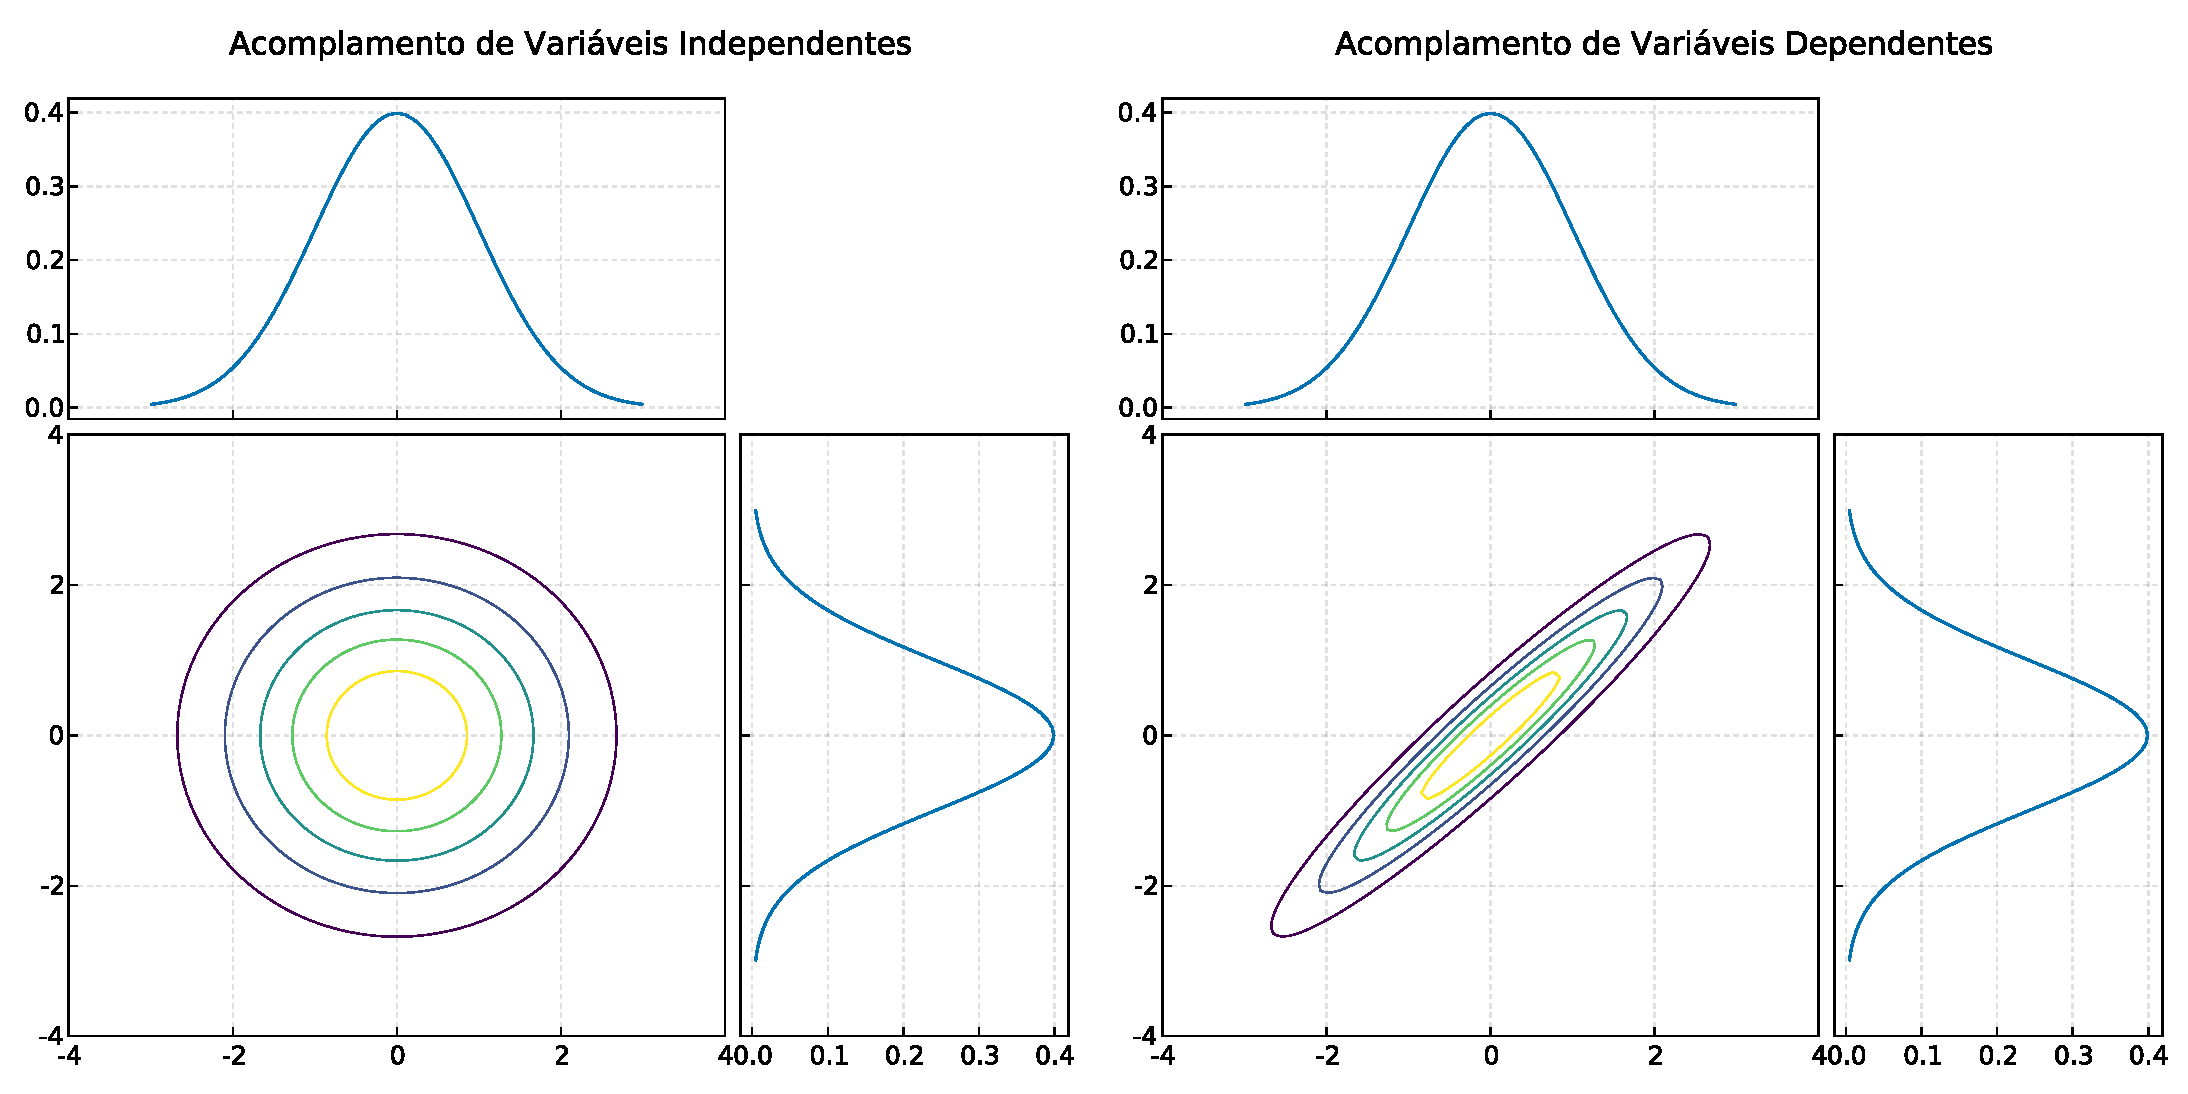
\includegraphics[width=0.7\textwidth]{Figures/coupling.pdf}
		\end{center}
		\caption{Exemplos de acomplamento.}
	\end{figure}

\end{frame}

\begin{frame}[fragile]{Teoria OT - Monge \& Kantorovich}

	\begin{definition}[Problema de Kantorovich]
		Dadas duas medidas de probabilidade $\mu \in \mathcal P(X)$,
		$\nu \in \mathcal{P}(Y)$ e a função de custo
		$c:X\times Y \to[0,+\infty]$, resolva:
		\begin{flalign}
			(KP)     &  &
			\inf
			\left\{
			\int_{X \times Y} c(x,y)d\gamma \ : \
			\gamma \in \Pi(\mu,\nu)
			\right\} &  &
			\label{eq:KP2}
		\end{flalign}
		\label{def:KP}
	\end{definition}

\end{frame}

\begin{frame}[fragile]{Teoria OT - Problema Dual}

	O Problema de Kantorovich tem uma formulação dual, que
	para certas condições de regularidade possui a mesma
	solução ótima que o problema primal (dualidade forte).

	\begin{definition}[Problema Dual]
		Dadas $\mu \in \mathcal P(X)$, $\nu \in \mathcal P (Y)$ e
		custo $c:X \times Y \to \mathbb R_+$. O
		Problema Dual é
		\begin{flalign}
			\mathrm{(DP)} &  &
			\sup \left \{
			\int_X \phi \ d\mu + \int_Y \psi \ d\nu \ :
			\phi \in C_b(X) \ , \psi \in C_b(Y) \ ,
			\ \phi \oplus \psi \leq c
			\right \}
			              &  &
			\label{eqt:dualproblem}
		\end{flalign}
	\end{definition}

	Funções $\phi, \psi$ são chamdas de \textbf{Potenciais de Kantorovich}.
	Essa formulação é utilizada nas Wasserstein GANs.

\end{frame}

\subsection{Distância de Wasserstein}
\begin{frame}[fragile]{Teoria OT - Distância de Wasserstein}

	\begin{definition}[Distância de Wasserstein]

		Seja $(X,d)$ um espaço métrico polonês, com $c:X \times X \to \mathbb R$ tal que $c(x,y)=d(x,y)^p$, e
		$p \in [1,+\infty)$.
		Para $\mu,\nu \in \mathcal P_p(X)$, a distância de Wasserstein é dada por:
		\begin{equation}
			W_p(\mu,\nu) :=
			\left(
			\inf_{\gamma \in \Pi(\mu,\nu)}
			\int_{X \times X} d(x,y)^p \ d\gamma
			\right)^{1/p}
			\label{def:Wasserstein}
		\end{equation}
	\end{definition}

	$\mathcal P_p(X)$ é o espaço de medidas de probabilidade com $p$-ésimo momento.

\end{frame}

\subsection{Distância de Wasserstein}
\begin{frame}[fragile]{Teoria OT - Distância de Wasserstein}

	A distância de Wasserstein preserva a geometria do espaço
	no qual está definida a medida.

	\begin{figure}[H]
		\centering
		\def\svgscale{0.45}
		\includesvg[inkscapelatex=false]{Figures/wasserstein-jsd.svg}
		\caption{Comparação entre a distância de Wasserstein e Jensen-Shannon.}
		\label{fig:pub}
	\end{figure}

\end{frame}

\subsection{Distância de Wasserstein}
\begin{frame}[fragile]{Teoria OT - Distância de Wasserstein}

	Dadas duas medidas de probabilidade $\mu$ e $\nu$,
	como então computamos a distância de Wasserstein
	entre elas?

\end{frame}

\subsection{Variações da Distância de Wasserstein}
\begin{frame}[fragile]{Teoria OT - Variações da Distância de Wasserstein}

	Calcular a distância de Wasserstein em espaços de alta dimensão (e.g. imagens)
	é bastante custoso.

	\vspace{3mm}
	Assim, variações da distância
	de Wasserstein foram desenvolvidas, como por exemplo:
	\begin{enumerate}
		\item Entropic Wasserstein;
		\item Sliced Wasserstein.
	\end{enumerate}

	\begin{figure}[H]
		\centering
		\def\svgscale{0.4}
		\includesvg[inkscapelatex=false]{Figures/entropic_ot.svg}
		\caption{
			Exemplo de solução de OT com regularização entrópica
			\citep{sales2021optimal}.}
		\label{fig:pub}
	\end{figure}

\end{frame}

\AtBeginSection{}
\section[Aplicações OT]{Aplicações de OT em Redes Neurais}
\subsection[WGAN]{Wasserstein GAN}
\begin{frame}[fragile]{Wasserstein Generative Neural Netorks}

	\textbf{Generative Adversarial Networks} (GAN)
	foram originalmente introduzidas por \citet{goodfellow2014}.
	Essas redes são utilizadas com o objetivo de gerar
	dados sintéticos realísticos a partir de dados reais.

	\begin{figure}[H]
		\centering
		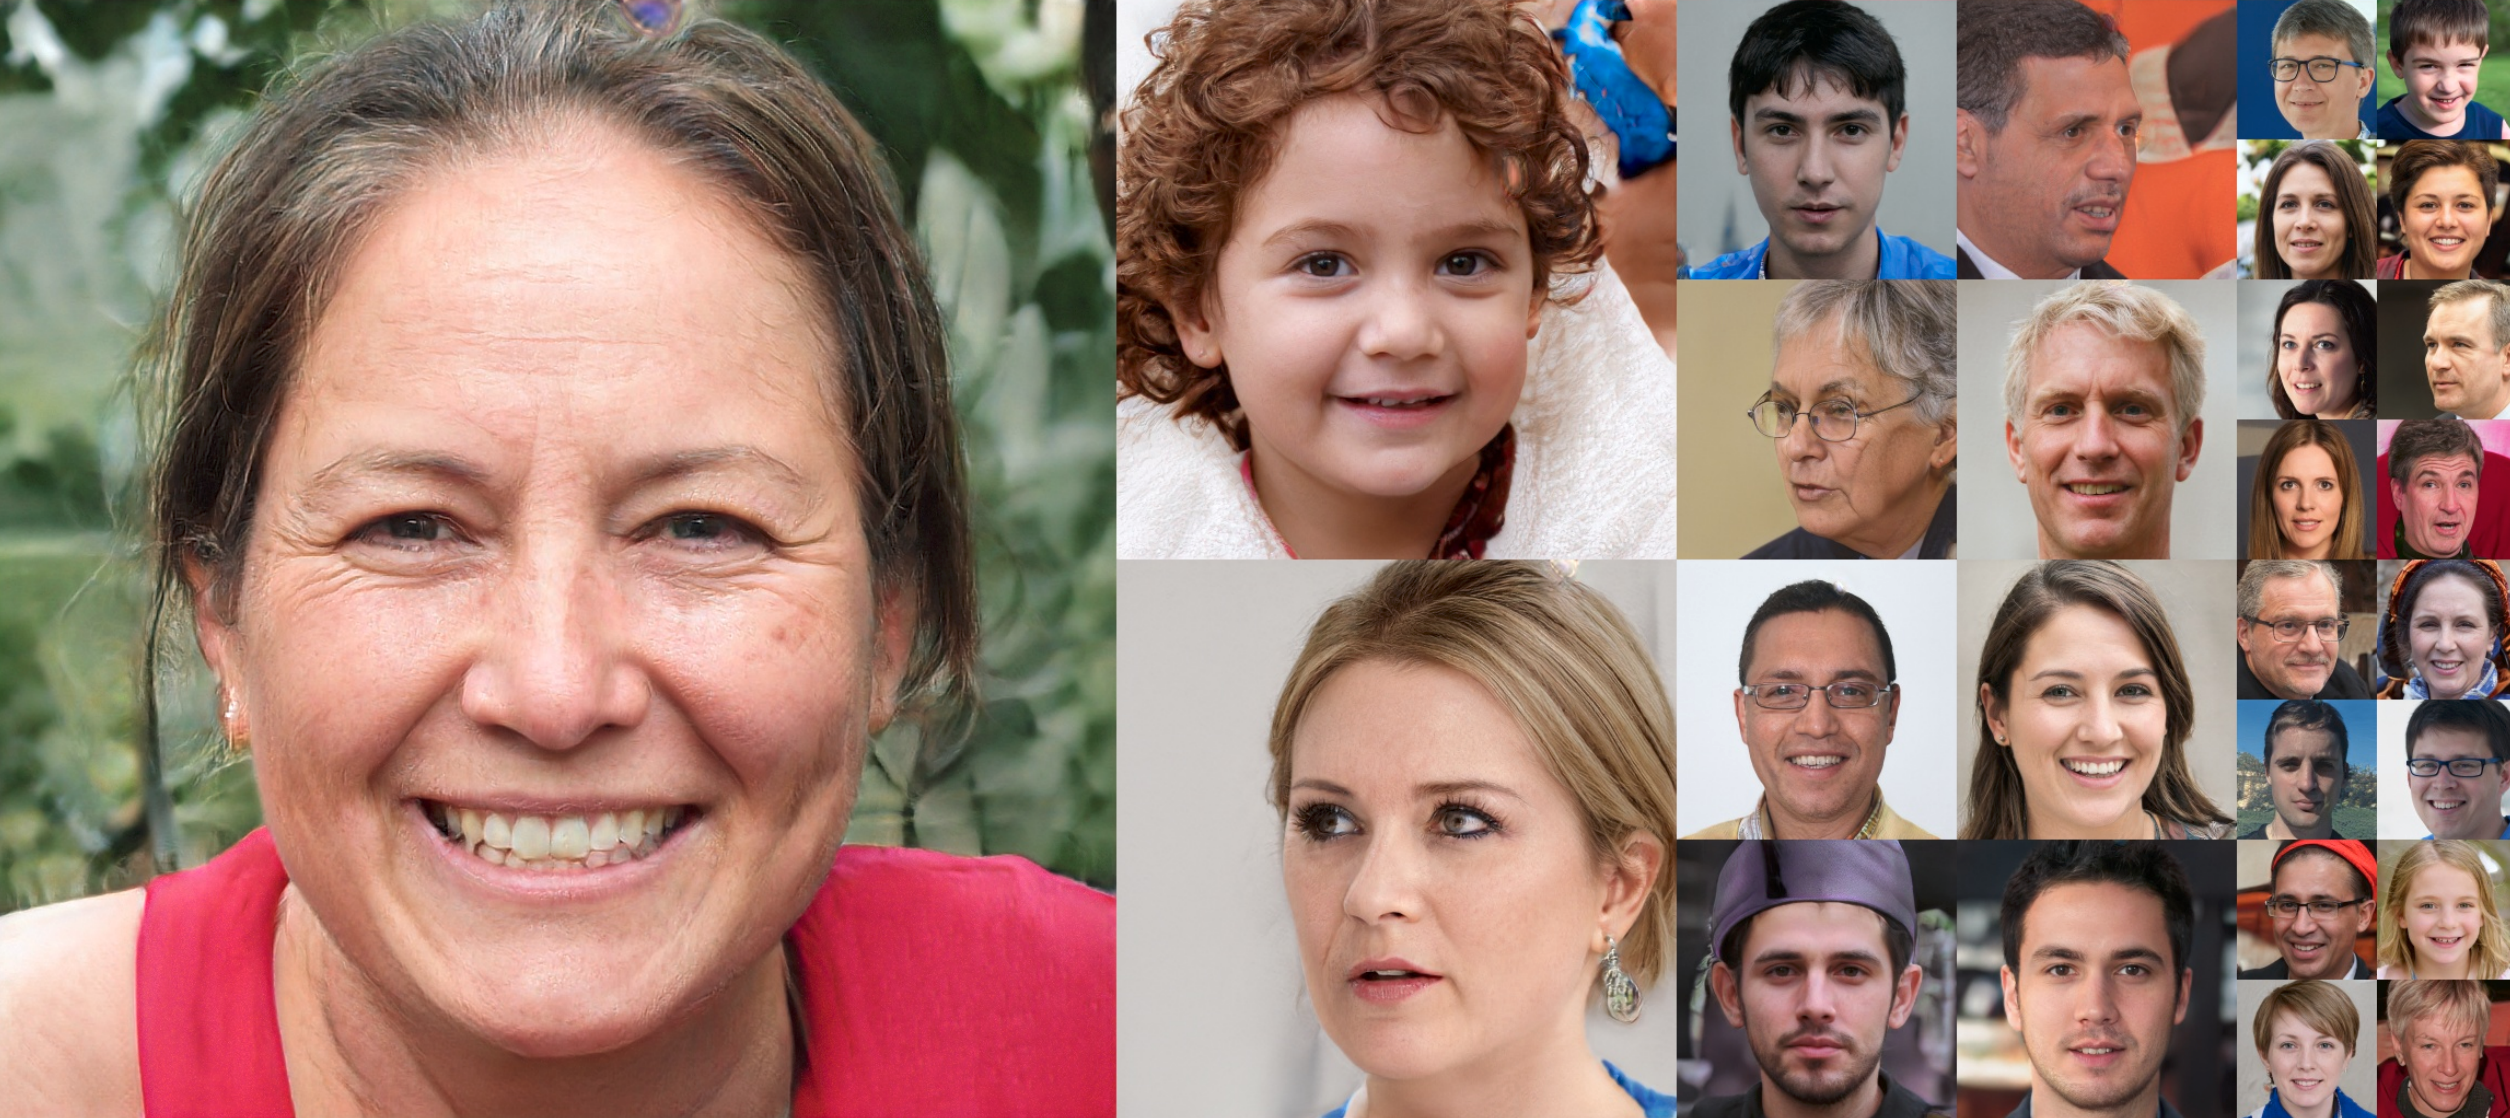
\includegraphics[width=8cm]{Figures/gans-faces.png}
		\caption{Faces geradas por GANs
			\footnote{Faces geradas por \citet{karras2018}}.}
	\end{figure}

\end{frame}

\begin{frame}[fragile]{Wasserstein Generative Neural Netorks}

	A ideia geral por trás das GANs é utilizar duas redes neurais
	competindo uma com a outra, sendo uma rede responsável por
	gerar amostras parecidas com os dados reais (\textit{gerador}) , enquanto a outra
	busca identificar quando o dado é real ou sintético
	(\textit{descriminador}).

	\begin{figure}[H]
		\begin{center}
			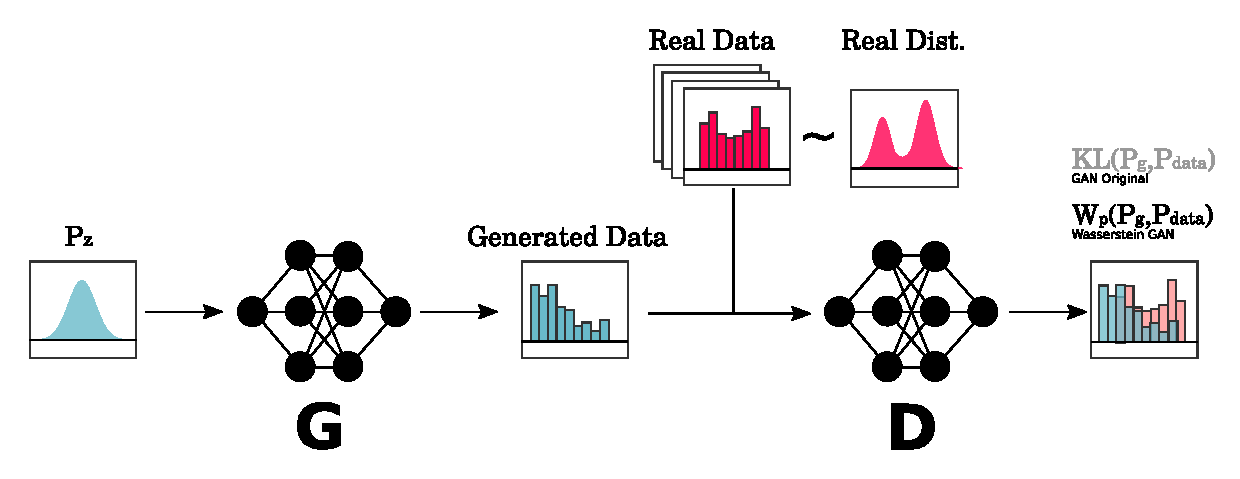
\includegraphics[width=1.0\textwidth]{Figures/wgan.pdf}
		\end{center}
		\caption{Generative Adversarial Network \citep{sales2021optimal}.}
	\end{figure}

\end{frame}



\begin{frame}[allowframebreaks]{References}
	\nocite{*}

	% \renewcommand{\bibsection}{\section{}}
	\renewcommand{\section}[2]{}%
	\tiny{\bibliography{ref}}
	\bibliographystyle{plainnat}
	% \bibliographystyle{plain}
	% \bibliographystyle{abbrv}
	% \bibliographystyle{apa}
\end{frame}


\end{document}
